\section{Methods}
\label{sec:methods}

\begin{figure*}[t]
  \centering
  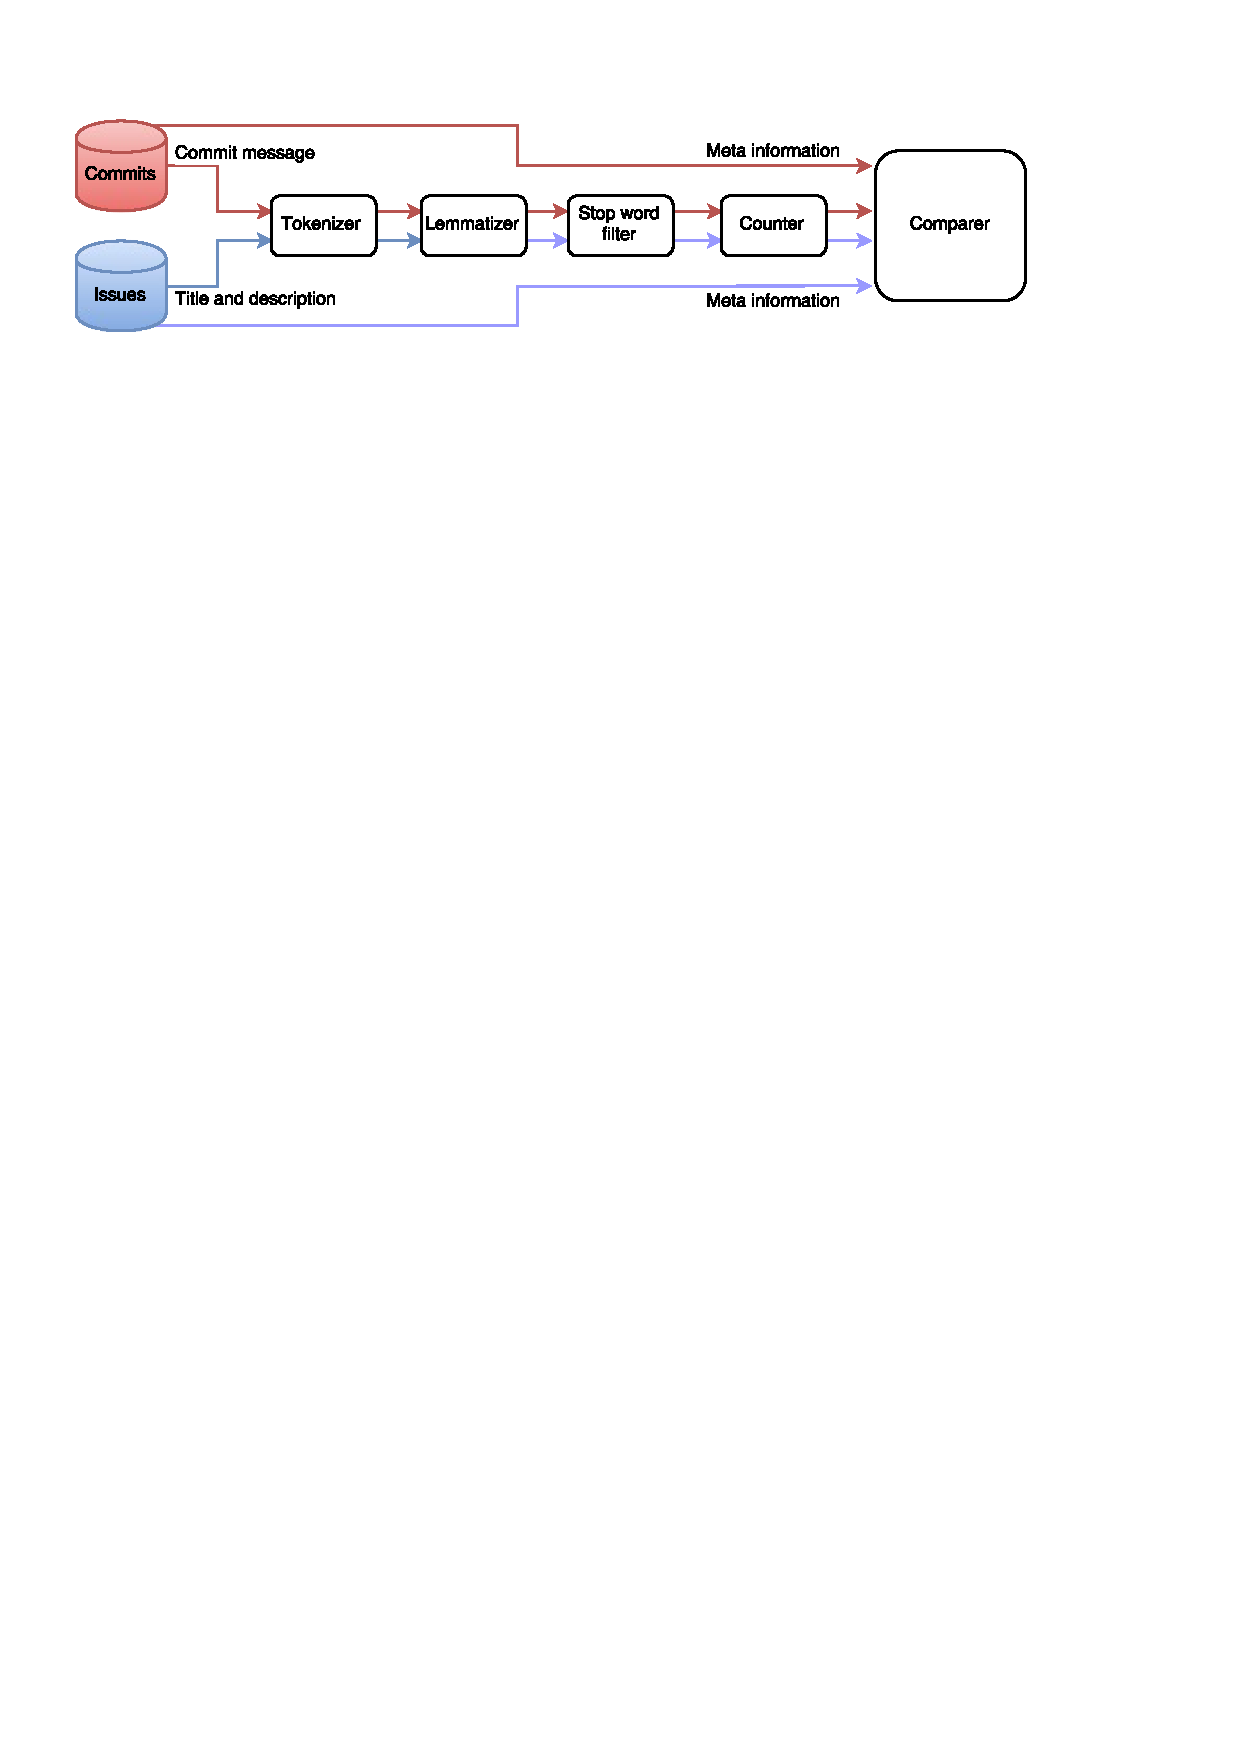
\includegraphics[width=\textwidth,trim={0 24cm 0 0},clip]{images/methods_vis.pdf}
  \caption{Pipeline of steps}
  \label{fig:methods_vis}
\end{figure*}

In order to find a relation between the commit messages and the issues, we need to start by reading the input data and tokenizing each commit message and the title and description of each issue into tokens.
In order to properly analyze natural languages, we need to lemmatize the tokens.
Lemmatization makes it possible to detect words that have the same meaning but appear differently in the text, either because of its tense (like ''walk'' and ''walked'') or because of the nature of that word (like ''good'' and ''better'').
Lemmatization normalizes every word so that we have one token for every word with the same meaning.
After the lemmatization step, we need to remove stop words so that only the interesting tokens are left.
The resulting tokens will then be placed in a table where the frequency of each token is stated for each commit message and issue.
Using this frequency table of tokens, we can compare the tokens of commit messages with the tokens of issues and find out the similarities based on the common tokens.
Figure \ref{fig:methods_vis} shows how these steps are to be processed one after another.


We also have access to the date, theme and the author for both commit messages and issues.
This kind of information can be useful when matching issues with commit messages.
For example, if a commit is done after an issue was submitted, it is less likely that the cause of this issue is related to that commit.
Similarly the theme and the author of commits and issues can help us classify the input and provide better results.
Grouping the commits and issues by their themes can increase the accuracy of matching and when the common words are not enough to determine a match, the system can provide a set of commits with a similar theme to the issue, instead of a single matching commit.
This might make it easier to find the commit manually, since the user has to only search a portion of the commits.

\subsection{Parsing}

\subsubsection{Parsing Issues}
Issues are provided as a .csv file, which is extracted from JIRA issue tracking system.
When we investigate the file, we realize that it follows the common .csv features and uses '';'' to separate the columns.
We have read and separated the values in our Java code and mapped it to an instance of our Issue class shown in Figure \ref{fig:issue}. 

\begin{figure}
\centering
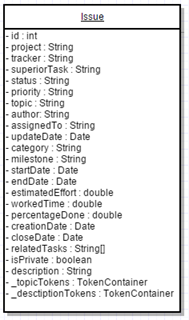
\includegraphics[scale=0.7]{issueClass}
\caption{Issue Java Class}
\label{fig:issue}
\end{figure}

One difference from a standard .csv format that the file exported from JIRA issue tracking system had was the additional description lines. Some issues have exception messages and log files attached to them to make it easier to describe the issue and provide further resources for the developer, who will fix the issue.
These descriptions contain multiple lines and thus a standard .csv parser cannot properly detect them.
Since the additional descriptions might be useful to understand more on what the issue is about, which is important for our case, we have implemented an additional functionality to detect these description lines and store them in our object.

We have created a regular expression shown in Figure \ref{fig:regexp} that detects whether a string is a new data record or not.

\begin{figure}
\centering
\verb/[0-9]+;[^\\n]+/
\caption{Regular Expression used to detect a new data record}
\label{fig:regexp}
\end{figure}

When reading each line of issue, we check the next line in the document before we move onto the next issue and we use the regular expression to determine whether this next line is a new issue or a line that contains additional description about the current issue.
If we detect additional description lines, then we also store them in the respective places in our java object.

Each issue object is then added to an ArrayList to store for further processing.

\subsubsection{Parsing Commits}

Commits are extracted from an SVN repository as a .txt file.
Each line in the file represents a single commit.
The information about the commit is separated by ''\#\#'' characters and each line is ended with ''\**'' characters.
Some commits also contain the duration of that particular task in the commit message, encoded by the ''@'' character followed by the time taken for that task.
An example line of commit can be seen in Figure \ref{fig:commitLine}.

\begin{figure*}
\centering
\verb/4013453##Markt Benedikt##Thu Feb 20 04:39:35 2014##Delete Button Problem bei Links umgangen refs #803 @1h\**  /
\caption{An example line of commit}
\label{fig:commitLine}
\end{figure*}

We have parsed each commit line in our Java program by separating them by ''\#\#'' characters, and then mapping them to an instance of our Commit Java class, shown in Figure \ref{fig:commit}.
We also detect the duration of each task by searching the ''@'' character inside the commit message.
The resulting Commit objects are then stored in an ArrayList for further processing.

\begin{figure}
\centering
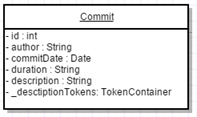
\includegraphics[scale=0.7]{commitClass}
\caption{Commit Java Class}
\label{fig:commit}
\end{figure}

\subsection{Tokenization}

When we set the description and the topic of an Issue object and the description of a Commit object, the input is immediately tokenized and stored in respective TokenContainer objects, which stores the tokens and their frequencies in a table like structure.

The tokenization process is done by separating each input text by whitespace characters.
The resulting words are stored in a TokenContainer and the TokenContainer is responsible for counting the frequencies of the words in the input text.
Later we can use the TokenContainer object to access every token and their frequencies.


\subsection{Lemmatization}

We use a library developed by Dr. Dipl. Inf. Ahmet Aker from University of Sheffield to do the lemmatization.
The library provides a functionality to determine the part-of-speech of a word and then it gives the lemma for that word given the correct part-of-speech.
The library has its own dictionary for part-of-speech tagging and lemmatization, and it supports English, German, Dutch, Spanish, Italian and French languages.

After getting the lemma for each word, we remove that token from our TokenContainer and instead insert the lemma as a new token.
This way different words that have the same lemma are counted as a single type of token and the frequency is also properly calculated. Some example words that are taken from the issue and commit messages and their corresponding lemmas are shown in Figure \ref{fig:lemma}.

\begin{figure}
\centering
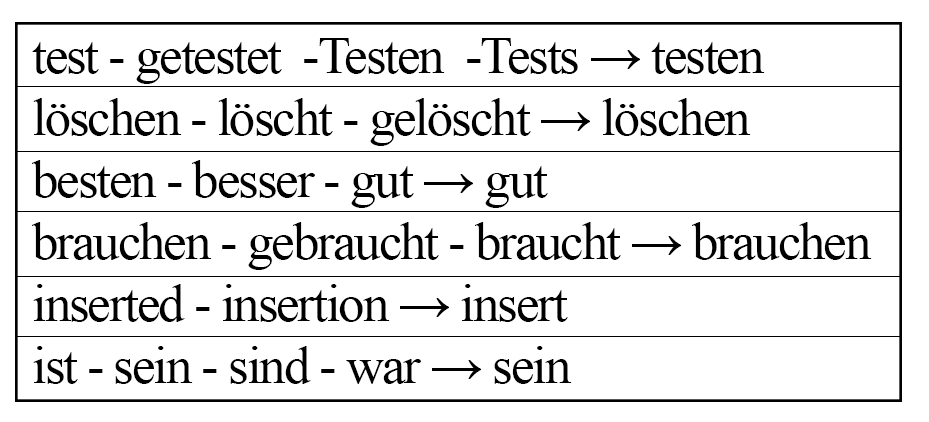
\includegraphics[scale=0.25]{lemmaExample}
\caption{Lemmatization examples from the issue and commit messages}
\label{fig:lemma}
\end{figure}

There are other lemmatization libraries, e.g. OpenNLP or StanfordNLP, but most of these libraries only offer English lemmatizers.
Our commit messages and issue descriptions are mostly German, so we looked for a tool with support for the German language.
There are only few free tools available on the web and even less which support the required language.
That is why we decided to choose the previously described library.
Probably the results would be more accurate if we had English commit messages and issue descriptions and we could have used a more distributed NLP tool for lemmatization.

\subsection{Mapping issues and commits}

Our aim is to connect each commit with at least one issue.
Given a table of lemmatized tokens and their corresponding frequency for both the commit messages and issue titles and descriptions we are able to calculate a first similarity value.\\
Each token in the issue table gets a rating based on its frequency.
If a token occurs less often it has a higher rating and if the token occurs in the issue title its value can get multiplied by a certain factor to give stronger weightings to the issue titles.\\
For each token from the commit message, we try to find the same token in the issue token table.
If there is a match we increase the similarity value of the relation of the commit and the issue the matching token corresponds to, by considering the token rating.
To not give relations a higher rating just because their descriptions, titles and commit messages consist of many tokens, we limit the number of tokens which add a value to the relation.
If we only consider a limited number of tokens with the highest rating we do not increase the similarity value of the relation each time there is any match but only for the rarest and most valuable tokens.
This means short titles, descriptions and commit messages will not get unfairly disadvantaged compared to those with more tokens.

Let's say for example that the token ''T1'' exists in the commit message of commit ''C1''.
The token ''T1'' also occurs in the issue title of the issue ''I1'' and in the issue description of the issue ''I2''.
We now have to create relations for ''C1'' and ''I1'' as well as for ''C1'' and ''I2''.
Both relations now have an initial similarity value depending on the frequency of ''T1'' and depending on whether ''W1'' occurs in the title or in the description (token rating).
The relation rating increases with each token match for a limited number of the highest rated tokens.

After calculating the relations based on the token similarity, we enrich the relation rating with some bonus points, which we calculate from meta information about the commits and issues.
Firstly, the relation gets bonus points if the closing date of the issue is very close to the commit date.
We assume that these bonus points are justified, because it is common practice to close an issue after it has been processed.
In a software project this is typically done by committing changes to the version control system.
So in the event that a new commit is done and an issue gets closed right after or right before we assume that there is a correlation between the commit and the issue.
Secondly, we compare the author of the commit with the person, who is assigned to the issue.
If the author of the commit matches the person, who is assigned to the issue, we add some bonus points to the relation, because it seems likely that in most cases the assigned person commits some issue related changes.

It is recalled that we already have a relation between an issue and a commit based on the token similarity when considering the meta information of issues and commits.
Hence there is the risk of adding bonus points to an wrongly assumed relation, which makes the result even worse.
On the other hand we would also have the chance of correcting false positives by reducing the relation rating if we see no correlation in the meta information.
Test runs with data from a real project can give insights about the usefulness of bonus points we discussed in this section.